\documentclass{article}
\usepackage[utf8]{inputenc}
\usepackage{amsmath}
\usepackage{amssymb}
\usepackage{color}
\usepackage{enumitem}
\usepackage{fancyhdr}
\usepackage[margin=1in,top=1in,headheight=18pt]{geometry}
\usepackage{listings}
\usepackage{graphicx}
\usepackage{hyperref}
\usepackage{dirtree}
\usepackage{tikzsymbols}
\usepackage{wrapfig}
\usepackage{subfig}
\usepackage{tikz}
\usepackage{soul}
\usepackage[toc,page]{appendix}
\usepackage[style=authoryear-icomp,maxbibnames=9,maxcitenames=2,backend=biber]{biblatex}
\addbibresource{./Authors.bib}
\graphicspath{ {./images/} }

\hypersetup{
    colorlinks=true,
    linkcolor=blue,
    filecolor=magenta,      
    urlcolor=cyan,
    pdftitle={Overleaf Example},
    pdfpagemode=FullScreen,
    }
    
\newcommand{\ExternalLink}{%
    \tikz[x=1.2ex, y=1.2ex, baseline=-0.05ex]{% 
        \begin{scope}[x=1ex, y=1ex]
            \clip (-0.1,-0.1) 
                --++ (-0, 1.2) 
                --++ (0.6, 0) 
                --++ (0, -0.6) 
                --++ (0.6, 0) 
                --++ (0, -1);
            \path[draw, 
                line width = 0.5, 
                rounded corners=0.5] 
                (0,0) rectangle (1,1);
        \end{scope}
        \path[draw, line width = 0.5] (0.5, 0.5) 
            -- (1, 1);
        \path[draw, line width = 0.5] (0.6, 1) 
            -- (1, 1) -- (1, 0.6);
        }
    }


\definecolor{ao}{rgb}{0.0, 0.0, 1.0}
\hypersetup{
    colorlinks=false,
}

\urlstyle{same}

\setlength{\parindent}{0pt}

\newcommand{\ttt}[1]{\texttt{#1}}

\title{Assignment 3 Part 2 - Speech Transcription}
\author{Introduction to Deep Learning \\ Emeritus \& Carnegie Mellon University}
\date{} \\
\vspace{.1in}

\begin{document}
\pagenumbering{arabic}

\maketitle

\section{Overview}
In this assignment, we'll be developing a model to transcribe audio directly to text.\\

In the first assignment, you did a similar task that involved identifying phonemes: units of speech. By contrast, your model in this assignment should directly produce readable text, complete with punctuation. \\

\textbf{Objective}: Given audio of human speech in the form of a spectrogram, produce a text transcription of what was said.\\

\textbf{Warning: This assignment is much more difficult than previous ones.} Not only are the pipeline and model complicated, but the training process can be unstable. The code will be surprisingly straightforward, but the concepts are difficult.\\

\textbf{But completing this should be rewarding}. You'll have a line-by-line understanding of a recent state-of-the-art model in speech transcription, and you'll also learn key concepts that appear in transformers and many other recent architectures. \\

\newpage
%----------------------------
\section{Pipeline Overview}

The model and pipeline we'll use comes from the \href{https://arxiv.org/abs/1508.01211}{\underline{Listen, Attend, Spell (Chan, Jaitly, Le, Vinyals 2015) \ExternalLink}} paper. \\

It's an older architecture, but we selected it because it accurately depicts how difficult state-of-the-art model design is, and also introduces covers many key concepts. Concepts include \textbf{attention, seq2seq problems, encoder-decoder architectures, and teacher forcing}. \\

\begin{figure}[h]
\centering
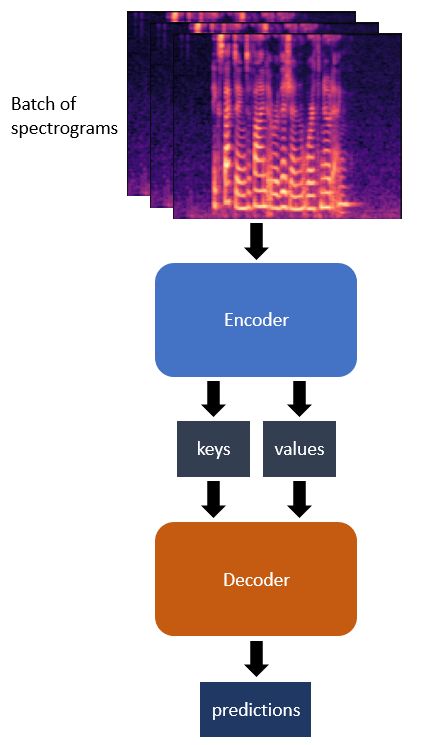
\includegraphics[width=0.4\textwidth]{images/pipeline.png}
\caption{Broad overview of LAS}
\end{figure}

Above is high-level view of LAS's architecture. \\

The main idea is pretty simple; we input a batch of spectrograms into the \textbf{encoder}. The goal of the encoder is to generate a condensed `summary' of the input that contains useful information for the decoder. The encoder returns two tensors (\textbf{keys} and \textbf{values}) that are given to the \textbf{decoder}. \\

The decoder's goal is to generate predictions of what's being said, token by token. Its output will be a \textbf{predictions} tensor shaped \ttt{(batch\_size, vocab\_size, max\_len)}. Basically, for each audio clip in the batch, we produce a sequence of logits. Each logit in the sequence indicates the probability that some character is at that position of the sequence. \\

The big picture is genuinely this simple. Of course, the devil is in the details, which we'll now cover.

% -----------------------

\subsection{Batching differently-sized elements}

Before we get to the encoder, an important question: how do you batch together multiple observations and/or labels that may differ in length? \\

\begin{figure}[h]
\centering
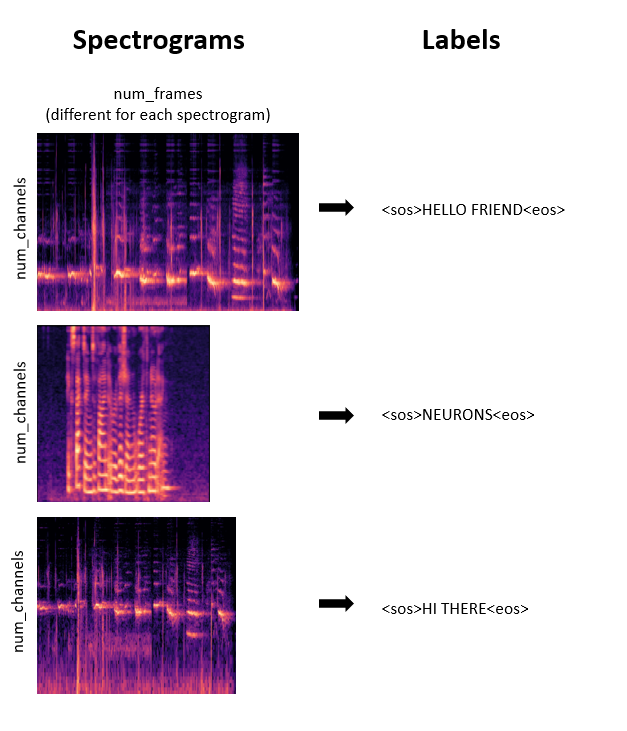
\includegraphics[width=0.7\textwidth]{images/spectrograms.png}
\caption{Multiple spectrograms and their labels.}
\end{figure}

Every spectrogram will have the same number of channels, but may differ in length. The spectrograms are each a tensor of shape \ttt{(num\_channels, num\_frames)}, where \ttt{num\_frames} varies.\\

The labels also vary in length. The labels begin and end with special tokens, marking the start and end of the sequence. Each label is converted to a 1D tensor, where each token is mapped to an integer index. So the first label in Figure 2 would be something like \ttt{[37, 8, 5, 12, 12, 15, 36, 6, 18, 9, 5, 14, 4, 38]}.\\

In the first two assignments of this course, we never had to worry about batches containing differently-sized elements; everything was the same size. All we had to do was stack each element along a new dimension, and we had a finished batch. \\

But these varying lengths make things harder.

\newpage

The simple solution is \textbf{padding}. \\

\begin{figure}[h]
\centering
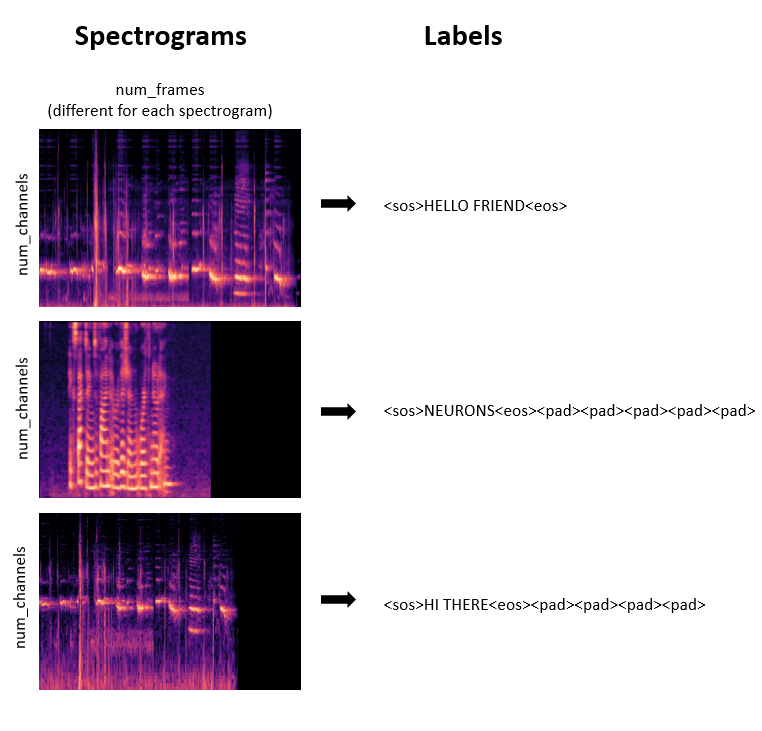
\includegraphics[width=0.75\textwidth]{images/spectrograms_padded.png}
\caption{Spectrograms and labels after padding. Note that \ttt{<sos>}, \ttt{<eos>}, and \ttt{<pad>} are single tokens.}
\end{figure}


While initializing your dataloader, you'll give it a \ttt{collate\_fn} (``collate function") that we wrote for you.

\begin{itemize}
    \item The \ttt{collate\_fn} tells the dataloader how to convert a list of observations into a single batch.
    \item In previous homeworks, we never had to write a custom \ttt{collate\_fn}, and so it used a default one that assumes everything is the same size, and just concatenates along a new axis.
    \item Our method pads the audio and labels to the same length, then concatenates and returns each of them.
    \item It also creates and returns \ttt{data\_lens} and \ttt{label\_lens} tensors, which will be needed throughout the pipeline.
\end{itemize}

% The \ttt{collate\_fn} tells the dataloader what to do spectrograms and labels and do the following:

% \begin{itemize}
%     \item Create a \ttt{lens} tensor that tracks how long each spectrogram was before padding. It should simply store a single integer (the \ttt{num\_frames}) per item in the batch. We'll need this during the decoder.
%     \item For \textbf{spectrograms}, make all spectrograms have the same length as the longest in the batch by \textbf{adding extra frames filled with 0's}, then concatenate them together along a new axis.
%     \item For \textbf{labels}, make all labels have the same length as the longest in the batch by \textbf{adding padding tokens (index 0 in our assignment)}, then concatenate them together along a new axis.
% \end{itemize}

% This \ttt{torch} function handles both padding and concatenating results into a single tensor: \href{https://pytorch.org/docs/stable/generated/torch.nn.utils.rnn.pad_sequence.html}{\underline{\ttt{pad\_sequence()} \ExternalLink}}. Just make sure you specify the arguments properly; this is a common source of bugs.\\

Hopefully not too bad so far!

%-----------------------

\newpage{}
\section{Encoder (``Listener")}

Now onto the actual model.\\

The goal of the encoder in this paper is to extract useful information from the audio input. For this reason, this paper sometimes calls the encoder the ``Listener"\footnote{``Listener" is not a general nickname for encoders; it's specific to this paper}. \\

\begin{figure}[h]
\centering
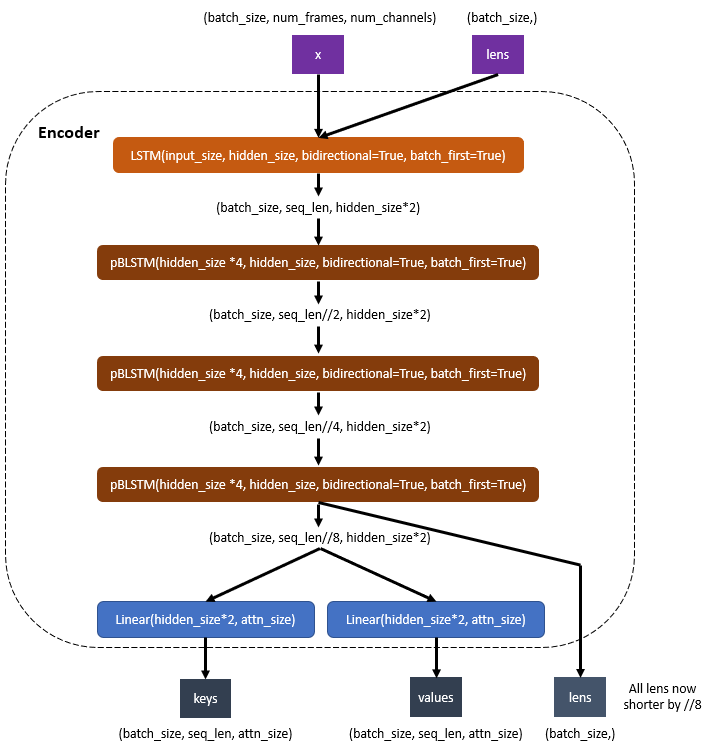
\includegraphics[scale=0.9]{images/encoder.png}
\caption{Encoder architecture}
\end{figure}

First, take a look at the initial plain LSTM layer of the encoder. Some notes:

\begin{enumerate}
    \item The \ttt{batch\_first=True} parameter tells the layer to input/output tensors with the \ttt{batch\_size} dimension first\footnote{For complicated CUDA-related reasons, RNN-based modules have the \ttt{seq\_len} dimension first, but nowadays most components expect \ttt{batch\_size} first, so we do this for consistency with previous assignments.}.
    \item The output has \ttt{hidden\_size*2} because \ttt{bidirectional=True}. Read the docs for \ttt{nn.LSTM} for why.
\end{enumerate}

\newpage

\subsection{pBLSTMs}

The encoder uses custom layers called \textbf{pBLSTM}s (``Pyramidal Bidirectional LSTMs"). \\

The main goal of each \ttt{pBLSTM} is to \textbf{downsample the length of a given input by half}. The encoder has 3 \ttt{pBLSTM} layers total, so after passing through all three layers, the data will have \ttt{seq\_len//8} (because $\frac{1}{2}^3=\frac{1}{8}$).\\

But note that they do more than just compression; they'll also be manipulating the values of the data.

\subsubsection{Downsampling?}

Question: Why downsample the input? \\

Answer: we downsample to make the information denser and more accessible to the decoder. \\

Reasons:

\begin{enumerate}
    \item Not every frame and not all parts of every frame will be useful
    \begin{itemize}
        \item E.g. silent frames or silent frequencies in frames
    \end{itemize}
    \item The number of frames is likely much larger than the length of the final text output
    \begin{itemize}
        \item Without downsampling, the decoder would need to look at a huge number of frames to generate just a single character
    \end{itemize}
\end{enumerate}

To illustrate, let's say we had a spectrogram of 200 frames of someone saying ``HELLO". Roughly speaking, this means there are around \ttt{200/5=40} frames we need to look at in order to generate a single character. But if we downsample to \ttt{200/8=25} frames, we only look at around \ttt{25/5=5} frames per character.

\subsubsection{Implementation}

Implementing the \ttt{pBLSTM} is surprisingly simple. It's just a wrapper around a bidirectional LSTM that handles downsampling.  \\

Here's the pseudocode:

\begin{enumerate}
    \item If there are currently an odd number of frames, throw away the last frame to end up with an even number\footnote{We can safely throw away this frame because it's unlikely to carry critical information, especially because it's at the end.}. This is needed for the next step.
    \item \ttt{reshape()} the input from \ttt{(batch\_size, seq\_len, hidden\_size)} to \\ \ttt{(batch\_size, seq\_len//2, hidden\_size*2)}
    \item Give the reshaped input to the BiLSTM, return the output
\end{enumerate}

That's it. Not too bad. \\

%-----------------

\newpage

\subsubsection{Optional Note: Reshaping?}

You can interpret the reshaping as moving some frames onto the \ttt{hidden\_size} dimension. 

\begin{figure}[h]
\centering
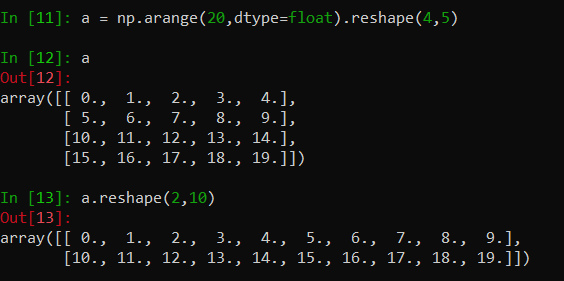
\includegraphics[scale=0.9]{images/reshaping.png}
\caption{Downsampling via reshaping example}
\end{figure}

Here's a simple visual example of this, assuming \ttt{(batch\_size=1, seq\_len=4, hidden\_size=5)}. After reshaping, every second ``frame" got moved onto the hidden dim of its predecessor. \\

The Bi-LSTM in the \ttt{pBLSTM} then ``mixes up" the information. And because the output size is smaller than the input size, it's forced to ``compress" it.

\subsubsection{Optional Note: Layer sizes?}

Hopefully you noticed a few odd details about the \ttt{pBLSTM} layer sizes. Here is their derivation.

\begin{itemize}
    \item Why the input size of \ttt{hidden\_size*4}?
    \begin{itemize}
        \item Recall from the encoder diagram the initial plain \ttt{BLSTM} layer that outputs a tensor with \ttt{hidden\_size*2}.
        \item Our first \ttt{pBLSTM} layer then performs the reshaping, which again multiplies that dimension by 2, resulting in \ttt{hidden\_size*4}, the exact size the layer is expecting.
    \end{itemize}
    \item Why the output size of \ttt{hidden\_size}?
    \begin{itemize}
        \item Because the \ttt{pBLSTM} is bidirectional, specifying an output size of \ttt{hidden\_size} will actually yield \ttt{hidden\_size*2} features, just like we said on page 5.
        \item This means that, each \ttt{pBLSTM} layer outputs the same number of hidden features as it received. However, the sequence length got halved.
    \end{itemize}
    \item As a result, all layers can have the same sizes, yet still manage to compress the input sequence.
\end{itemize}

It's definitely possible to do downsampling in other ways too!


\newpage
%------------------------

\subsection{Key Network and Value Network}

The final part of the encoder is two \textbf{separate} linear layers: the \ttt{key\_network} and \ttt{value\_network}. You'll need to give the output of the last \ttt{pBLSTM} to each of these layers in order to get the \ttt{keys} and \ttt{values}. \\

Notice that the \ttt{keys} and \ttt{values} are essentially two different projections of the input. We make these to use for attention, which we'll explain on the next page.

\newpage
% ---------------


\section{Attention}

\textbf{Attention} is actually calculated during the decoder, but we'll introduce it now, so you don't have to juggle learning both the decoder and attention later on.

\subsection{Introduction}

Attention has become a very important concept in deep learning in the last few years. Most notably, transformers use it extensively in the form of self-attention and multi-head attention (which we won't cover, but we encourage you to look up after completing this assignment). \\

Attention in deep learning is meant to loosely mimic how attention works in organic brains. When humans `pay attention' to something, they limit the amount of information they process and focus in on certain stimuli. This is believed to help cognition by allowing them to better allocate their finite computational resources and extract signal from noise. \\

A computational model of this is very useful in LAS. \\

The decoder works by predicting one token of the output at a time, using the encoder's summary of the input. But some parts of the input are more relevant to certain tokens than others. \\

For instance, if our decoder is near the end of a transcription, information near the very beginning of the input is probably not as important anymore. So we should ideally deprioritize it and focus more on the end of the input. This is what attention will help us do.

\subsection{Intuition: Queries, Keys, and Values}

Attention works by using three tensors called \ttt{query}, \ttt{keys}, and \ttt{values}. They're so named because attention kinda works like querying a database. \\ 

For example, say we're searching YouTube for a specific video:

\begin{itemize}
    \item You search for a video by typing out a string, which is your \textbf{query} to the YouTube database.
    \item The query gets compared to a set of \textbf{keys}, which are things like video titles, tags, description text, etc.
    \item If any keys match well with our query, the database returns the \textbf{values} (videos) that correspond to those keys.
\end{itemize}

The main idea is that this process allows us to filter out parts of the \ttt{values} that weren't relevant to our \ttt{query}. \\

Here's that same metaphor above, but in LAS terms:

\begin{itemize}
    \item The decoder will produce a \ttt{query} every time it wants to predict a token.
    \begin{itemize}
        \item This \ttt{query} is attempting to find parts of the input (from \ttt{values}, which is the encoder's summary of the input) that are relevant to its next prediction.
    \end{itemize}
    \item The \ttt{query} gets compared against the \ttt{keys} that the encoder had generated.
    \item We calculate \ttt{attention}, which represents how well each \ttt{key} matched our \ttt{query}. We then compare \ttt{attention} with \ttt{values}, which creates a tensor \ttt{context}.
    \begin{itemize}
        \item \ttt{context} is like the list of relevant videos YouTube would give you. It's the subset of information from \ttt{values} that we're paying attention to.
    \end{itemize}
\end{itemize}

We encourage you to review this description after seeing the next page, if needed.

% Let's now apply this database metaphor to the LAS decoder. The decoder wants to predict a token of the output, but we know only certain parts of the input will be relevant to this token.

% \begin{itemize}
%     \item The decoder creates a query, containing information about what tokens it predicted so far.
%     \item The query is compared against the keys that our encoder created.
%         \begin{itemize}
%             \item Recall that the keys are an ordered summary of the input.
%         \end{itemize}
%     \item If any keys match well with our query, the database returns the \textbf{values} (slices of the input) that correspond to those keys.
% \end{itemize}

% So how does this database metaphor apply to the decoder in LAS?\\

% Recall that the decoder's job is to predict the output sequence, one token at a time. When it's predicting a token, it needs to figure out which part of the input to attend to. \\

% For the decoder, the 

% Recall that the encoder outputs two summarized projections of the input: the \ttt{keys} and \ttt{values}. The decoder's job is to predict the final output sequence using certain parts of the input. The decoder only needs to pay attention to certain parts of the input in order.

\newpage

%------------------
\subsection{Implementing Dot Product Attention}

Now that we've covered the `why' of attention, let's discuss the `how'. \\

For LAS, we'll be implementing one of the simplest forms of attention in deep learning, called \textbf{dot product attention}.  \\

\begin{center}
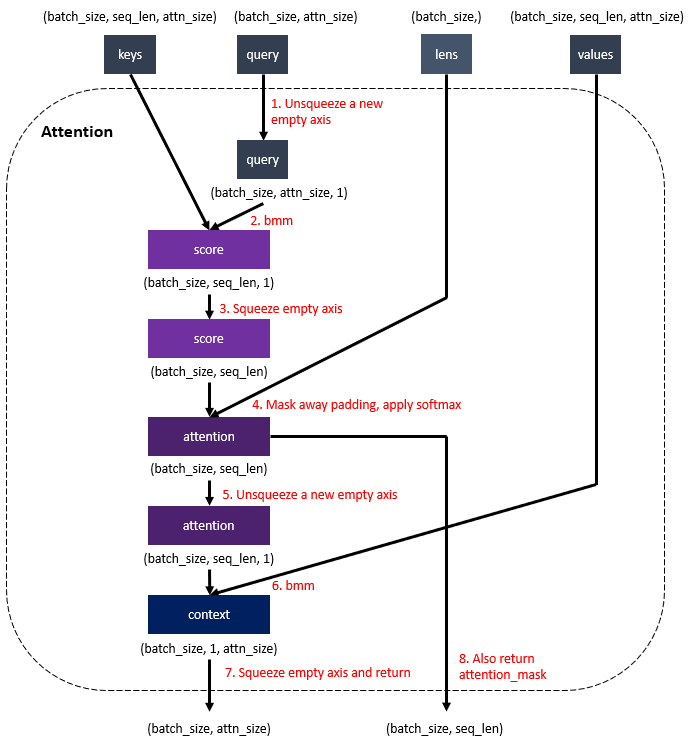
\includegraphics[scale=0.9]{images/attention.png}
\captionof{figure}{Attention pipeline}
\end{center}

In colloquial terms, we first compare the \ttt{keys} to the \ttt{query} to get \ttt{scores} of how well they match. We mask away any padding tokens, then scale the \ttt{scores} between 0 and 1 with a softmax, giving us our \ttt{attention}. Finally, we compare the \ttt{attention} with the \ttt{values} to get our final \ttt{context}. We also return the \ttt{attention} mask we generated, which we can use to monitor the network's training progress. \\

The diagram may look a little complex, but it's actually all you'll need to implement the code. We marked the steps of the pseudocode in red. Look up the \ttt{torch} methods for \ttt{unsqueeze}, \ttt{squeeze}, and \ttt{bmm}. \\

The code for step 4 is difficult to explain and not very insightful, so we'll just give it to you in the notebook. The goal of this step is to prevent attending to padding. We set the pre-softmax values of the padding to $-\infty$, which makes the post-softmax values close to 0. \\



\newpage
%-----------------





% For us, our \textbf{query} is the output of our \ttt{LSTMCell}s. We then \ttt{bmm} (``batch matrix multiply") it with our \textbf{keys} (each `key' is a slice of the input) and get an \textbf{attention mask}. The attention mask indicates the `strength' of the match. The final \ttt{bmm} between our mask and the \textbf{values} effectively `compares' the match between query/key and the values, and pushes irrelevant values to 0, while maintaining relevant ones. \\

% -------------
\newpage


\section{Decoder (``Speller")}

% The job of the decoder is to \textbf{generate the predicted output sequence} using the encoder's summary of the input. \\

The decoder is unfortunately much more complicated than the encoder - the encoder is a linear pipeline, but the decoder is \textbf{recurrent}. \\

Also, note that the \textbf{decoder works differently depending on if you're in training or eval mode, and whether you have teacher forcing or not}. For now, we'll introduce the decoder in training mode and discuss how eval and teacher forcing modify it.

% \subsection*{Important Note: Decoder Modes}

% Introducing the decoder is complicated because it can work in \textbf{3 different possible ways}. \\

% How it works depends on whether you're in training or eval mode, and whether you are \textbf{teacher forcing} during training or not. \\

% We'll introduce it in this order to make things clearer: 

% \begin{enumerate}
%     \item Training mode, no teacher forcing
%     \item Training mode, teacher forcing
%     \item Eval mode
% \end{enumerate}

% The first version is the most basic; we'll describe the other two by describing how they differ from the first. \\

% The differences between each mode aren't that complicated, don't worry. But it's important to understand them clearly; your code should be prepared to detect and work for all three modes.


% %------------------
% \newpage

\subsection{Decoder Overview}

The decoder's main job is to predict the appropriate output sequence using the encoder's summary of the input. \\

It does this by \textbf{predicting one token at a time, in order}. In other words, at \ttt{t=0}, given the start token, the decoder calculates \ttt{context} and predict the first token of the label. At \ttt{t=1}, the decoder uses the token it predicted previously to calculate \ttt{context} and  predict the next token, and so on. \\

Notice how this process resembles how humans write; we write one character at a time, while keeping in mind what we've written previously. \\

But at what \ttt{t} should it stop predicting new tokens? It stops when it predicts enough tokens to match the length of the longest label in the batch. In other words, it stops when \ttt{t=max\_len}, where \ttt{max\_len = seq\_len - 1}\footnote{The \ttt{-1} is because the start token is already given}.\\

\textbf{Summary:}

\begin{itemize}
    \item The main idea of the decoder is a \ttt{for} loop, that runs from \ttt{t=[0, ..., max\_len-1]}.
    \item At each \ttt{t}, the decoder will try to predict the next token using information about the previous token it generated and attended input.
\end{itemize}

% \newpage
% %----

\subsection{How the Decoder Makes Predictions}

Now for a high-level conceptual overview of what happens at each timestep of the \ttt{for} loop:

\begin{enumerate}
    \item Create an embedding of the previous token we generated
    \item Pass this embedding through two \ttt{LSTMCell}s
    \item Figure out which parts of the input to pay attention to (\ttt{context}), by using the output of the \ttt{LSTMCell}s as your \ttt{query} to the attention layer
    \item Predict the next character by concatenating the attended input and the output of the cells, and passing that through a linear layer to get logits.
    \item Save your prediction logit by appending it to a list.
\end{enumerate}

In short, at each timestep, we predict the next token given our previous predictions and the parts of the input that we're currently paying attention to. \\

Now for the implementation details.

\newpage
%------------

\subsection{Implementing the Decoder}

\subsubsection{Initialization}

We first initialize the following layers:

\begin{itemize}
    \item \ttt{nn.Embedding}
        \begin{itemize}
            \item This layer is basically a learned lookup table, mapping some index to a meaningful embedding vector. Essentially, it makes indices richer and more interpretable for deep learning.
        \end{itemize}
    \item Two \ttt{nn.LSTMCell}s
        \begin{itemize}
            \item Just like we did in part A of this assignment, we're going to be passing inputs and hidden states between cells and between time steps.
        \end{itemize}
    \item \ttt{Attention} layer to attend to input
    \item \ttt{nn.Linear} to predict the next token
\end{itemize}

\subsubsection{Preparing for the \ttt{for} Loop}

The decoder's forward pass receives the \ttt{keys}, \ttt{values}, and \ttt{lens} tensors from the encoder. \\

It then does the following to prepare for the \ttt{for} loop:

\begin{enumerate}
    \item Set \ttt{max\_len = seq\_len - 1}
    \item Initialize \ttt{prediction} tensor, shaped \ttt{(batch\_size, vocab\_size)}.
        \begin{itemize}
            \item During the \ttt{for} loop, this will be our logits that represent our prediction of the next char at each iter.
            \item However, since we haven't predicted anything yet, we set it as if it is predicting \ttt{<sos>}, since we always know the \ttt{<sos>} token comes first.
        \end{itemize}
    \item Initialize \ttt{context} tensor, shaped \ttt{(batch\_size, attn\_size)}, by taking it from the first timestep of the \ttt{values} tensor.
        \begin{itemize}
            \item During the \ttt{for} loop, this tensor will abstractly store information about previous characters we've predicted.
        \end{itemize}
    \item Initialize some empty lists:
        \begin{itemize}
            \item \ttt{predictions}, where we'll append the logit for each token we predict. At the end of the \ttt{for} loop, it should contain \ttt{max\_len} tensors. Later, we'll concatenate this list into a single tensor and give that to our loss function.
            \item \ttt{hidden\_states}, the hidden states of the two \ttt{LSTMCells} that create the attention query for each timestep 
            \item \ttt{attentions}, to store the attention mask produced at each time step. Saving these is optional but recommended; we can visualize them later to make sure our network is learning properly.
        \end{itemize}
\end{enumerate}

It's a lot to take in, so don't worry if it's not 100\% clear yet. The next section should help explain why we declared all of those variables.

%-------------
\newpage

\subsubsection{The \ttt{for} Loop}

This is the prediction algorithm we described in 5.2, but with technical details. 

\begin{enumerate}
    \item Create embedding of previous token \ttt{x}, that's the input tensor for the \ttt{LSTMCell}s
        \begin{enumerate}
            \item Identify the indices of the tokens we predicted in the previous timestep by taking the \ttt{prediction} vector and applying \ttt{argmax} along its \ttt{vocab\_size} dim. This creates a batch of indices shaped \ttt{(batch\_size,)}. Pass these to your embedding layer, to get a \ttt{char\_embed} tensor
            \item Concatenate \ttt{char\_embed}
            \ttt{(batch\_size, hidden\_size)} and \ttt{context} \ttt{(batch\_size, attn\_size)} along the appropriate dimension to get \ttt{x} \ttt{(batch\_size, hidden\_size+attn\_size)}
        \end{enumerate}
    \item Pass \ttt{x} through the \ttt{LSTMCell}s
        \begin{enumerate}
            \item Give the first cell \ttt{x} and \ttt{hidden\_states[0]}. Store the output in {hidden\_states[0]}. Set \ttt{x} to be \ttt{hidden\_states[0][0]}
            \item Give the second cell \ttt{x} and \ttt{hidden\_states[1]}. Store the output in {hidden\_states[1]}. Set \ttt{x} to be \ttt{hidden\_states[1][0]}
        \end{enumerate}
    \item Give appropriate arguments to attention, using \ttt{x} as the \ttt{query}. It will return \ttt{context} and \ttt{attention}
    \item Concatenate \ttt{x} and \ttt{context} along the \ttt{hidden\_size} dimension. Give this to your linear layer to get \ttt{predictions}
    \item Store your results by appending \ttt{prediction} to \ttt{predictions} and appending \ttt{attention[0, :]} to \ttt{attentions}
    \begin{itemize}
        \item The reason for the \ttt{[0, :]} indexing on \ttt{attention} is to grab only the first item in the batch. We only need one per timestep for visualization purposes
    \end{itemize}
\end{enumerate}

That's it for the \ttt{for} loop. \\

Make sure to look up the official documentation for each method you use. Otherwise, try not to overthink each individual step; we streamlined this process to make it less ambiguous.

\subsubsection{Returning Results}

To wrap things up, we need to combine our \ttt{predictions} and \ttt{attentions} and \ttt{return} them. \\

\ttt{torch.stack} your \ttt{predictions} along a new \ttt{dim=2} axis to get \ttt{(batch\_size, vocab\_size, max\_len)}. Also, \ttt{torch.stack} the \ttt{attentions} along a new axis \ttt{dim=0} to get \ttt{(max\_len, seq\_len)}. Return both. \\

You're almost done with the decoder, but there's two last implementation details we need to cover.

\newpage
%----

\subsection{Teacher Forcing}

We mentioned earlier that \textbf{teacher forcing} affects the implementation of the decoder.\\

Teacher forcing is a technique used during training to dramatically improve performance. It's basically mandatory for this assignment; if you don't implement it, your decoder may never even converge. \\

The main idea is \textbf{to embed the label token instead of the token it predicted previously some percentage of the time}. In other words, if \ttt{tf\_prob=0.9}, with 90\% probability we will provide the label instead of our previous prediction at each timestep. \\

The reason this helps is because the decoder will be awful when you first begin training. Because each prediction relies on the quality of previous predictions, having very poor quality predictions means it'll take ages to improve, if it ever does.

\subsubsection{Implementing Teacher Forcing}

Fortunately, the implementation is simple, with minimal changes.

\begin{itemize}
    \item (Given) While preparing for the \ttt{for} loop, generate embeddings for the labels in advance to save on computation time
    \begin{itemize}
        \item Pass \ttt{labels} through the \ttt{embedding\_layer} to get \ttt{label\_embeddings} shaped \ttt{(batch\_size, max\_len+1, hidden\_size)}
    \end{itemize}
    \item In the \ttt{for} loop pseudocode, modify step 1a by checking if some random float between 0 and 1 is lower than the \ttt{tf\_prob}
        \begin{itemize}
            \item If so, set \ttt{char\_embed} as \ttt{label\_embeddings[:,t,:]}.
            \item Else, embed your previous prediction, just like normal
        \end{itemize}
    \item When training, make sure you give the model a non-zero \ttt{tf\_prob}. Conversely, during eval, make sure \ttt{tf\_prob} is its default value, zero. 
\end{itemize}

\subsubsection{Rate and Scheduling of Teacher Forcing}

Now for a critical question: \textbf{what \ttt{tf\_prob} should you use?} \\

The answer is to \textbf{around 90 to 95\%}. You can optionally begin to lower this number by 0.5\% or 1\% per epoch after attention begins to converge. \\

The reason this high rate helps is because it lets your decoder initially focus on learning how to spell. And gradually decreasing it after it begins to converge coaxes the model into relying on its own previous predictions. After it becomes a decent speller, it'll start taking into account the encoder information in order to further lower the loss.


\subsection{Eval Mode}

Eval also affects the implementation of the decoder. \\

It's fortunately very simple:

\begin{itemize}
    \item (Given) \ttt{max\_len} should be some reasonable length given typical labels in the dataset (we set it as 600)
    \item \ttt{labels} should be None (default value)
    \item \ttt{tf\_prob} must be 0 (default value)
\end{itemize}

No changes to your model code are necessary, as we already gave you the first item and the other two only matter in your training and eval loops. Just be aware of these differences.

\newpage
%-----------

\section{Training and Evaluating LAS}

Some final important notes.

\subsection{Training}

\begin{itemize}
    \item Follow the teacher forcing scheduling in 5.4.2. It will be critical to passing the assignment.
    \item Mixed precision from the previous assignment probably won't cause much speedup; the time bottleneck is in the sequential nature of the LSTMs and decoder.
    \item We recommend you use \href{https://pytorch.org/docs/stable/generated/torch.nn.utils.clip_grad_norm_.html}{\underline{gradient clipping \ExternalLink}} to prevent exploding gradients from harming training.
    \item If you choose to use LR scheduling, don't activate it until attention starts to work. This may take anywhere between 10 to 30 epochs.
    \item Each epoch will probably take between 10 to 25 minutes.
    \begin{itemize}
        \item If your code is much slower, make sure that you're using a GPU and that your dataloader settings are adequate (particularly \ttt{num\_workers}). If those two are correct, try to identify and address the speed bottleneck in your code.
    \end{itemize}
    \item Training will be unstable.
    \begin{itemize}
        \item It's common to observe slow decreases in loss and poor eval performance for 10-20 epochs, then a sudden improvement.
        \item Unfortunately, this can make it hard to tell if your network is bugfree and actually working.
        \item One way to tell your network is working is by monitoring \textbf{attention plots}, which we'll introduce on the next page
    \end{itemize}
\end{itemize}

\newpage
%---------------

\subsubsection{Attention Plots}

Visualizing attention of a single utterance once per epoch is a good way to gauge training progress. \\

% \begin{center}
%     \includegraphics[scale=1]{images/trained_attention_example.png}
%     \captionof{figure}{Example of a decent model's attention plot}
% \end{center}

\begin{figure}[h]
    \centering
    \subfloat[\centering Untrained model's attention plot]{{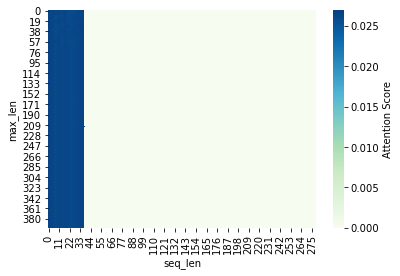
\includegraphics[width=0.33\textwidth]{images/untrained_attention_example.png}}}%
    % \qquad
    \subfloat[\centering Trained model's attention plot (short example for clarity, no padding)]{{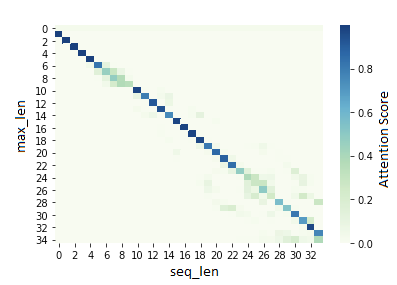
\includegraphics[width=0.33\textwidth]{images/trained_attention.png}}}%
    \subfloat[\centering Trained model's attention plot (realistic example, padding)]{{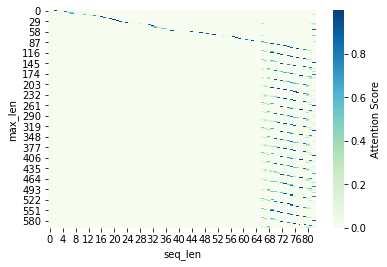
\includegraphics[width=0.33\textwidth]{images/trained_attention_padding.png}}}%
    \caption{Examples of attention plots}
\end{figure}

\begin{itemize}
    \item The leftmost image is a bad attention plot of an untrained model. The center and right image are good plots of trained models.
    \item Interpretation: ``during each timestep, which part of the summarized input did the decoder pay attention to?"
    \begin{itemize}
        \item \ttt{seq\_len} is the length of the padded spectrogram after being shortened by the encoder by a factor of 8.
        \item \ttt{max\_len} is the number of timesteps in the decoder.
    \end{itemize}
    \item A decent model's attention plot should have a distinct diagonal line that starts at the top left corner.
    \begin{itemize}
        \item As seen in the last image, padding causes weird behavior, but this is perfectly fine because it doesn't matter anyway.
        \item It also doesn't have to go to the bottom right corner, nor be be perfectly diagonal, nor be perfectly clear. This is also fine.
    \end{itemize}
    \item Notice the values range between 0 and 1. This is due to the softmax used to calculate attention. The higher the value, the more attention was paid.
\end{itemize}

Hopefully you can see why having a diagonal line is good. The beginning of your audio is likely relevant to the first few characters you generate, same for the middle, same for the end. Assuming a model is using the audio input properly, the attention will form this pattern.\\

\textbf{For the first 5 to 20 epochs, the plots will probably be pretty poor, despite train loss decreasing.} This is normal; your model is likely learning how to spell first, without paying much attention to the input. After it gets decent and \ttt{tf\_prob} starts to gradually decrease, it'll start learning to interpret the input, which is when the performance will suddenly improve. \\

We wrote a method that creates and saves an attention plot for you in \ttt{utils.py} called \ttt{plot\_attentions}. We recommend you save an attention plot once per epoch, to get a gauge on how it's doing.

\newpage
%-------------------

\subsection{Evaluation}

Last section.

\begin{itemize}
    \item We recommend you use a metric called  \href{https://en.wikipedia.org/wiki/Levenshtein_distance}{\underline{Levenshtein distance \ExternalLink}} to gauge your model's performance.
    \begin{itemize}
        \item In short, it measures how different your predicted string is from the true label. The higher the distance, the worse your prediction is.
        \item Make sure to run the cell in the beginning of the notebook that installs the \ttt{python-Levenshtein} library.
    \end{itemize}
\end{itemize}

\noindent\rule{\textwidth}{1pt}

You're done with the writeup! See you in the notebook!


% Next, we pass this input through two LSTM cells. Then, the LSTM output is used to calculate a context using attention. Lastly, we pass the LSTM output and the context through a linear layer to get a prediction distribution. We can take the argmax of this distribution to get a predicted character, and then start the process over for the next character to predict. Before we go more in depth, here's a diagram of this: \\

% \begin{figure}[h]
% \centering
% 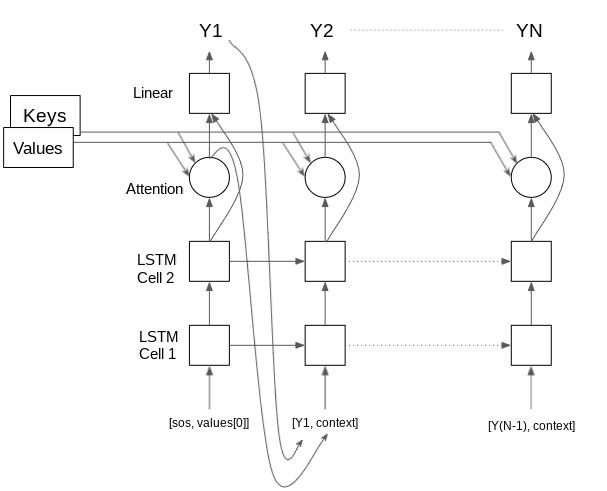
\includegraphics[scale=0.53]{images/decoder_old.png}
% \caption{The Speller Architecture for LAS}
% \end{figure}

% Now let's go more in depth:\\

% \subsection{Sequence Length and Input Characters}

% First, we're going to have to figure out how many characters we want to predict. During training, we can simply use the max length of the labels. However during inference, we will want to use some hard coded value, like 600, since we don't know how long the text is.\\

% We will also want to know what characters to input at the bottom of the decoder (see Figure 4). During training, for the first character, we will always want to use "SOS", for "start of sequence" (see utils.py to see what index this is). However in training it's less clear what we should use for the second time around. Should we input the prediction for the first character, or should we use the label for the first character? Start off by using the label, for debugging, but once that works, use the label with 90\% probability, and the previous prediction with 10\% probability. During inference, you will always use the previous prediction.

% \subsection{Passing Input Through the LSTM Cells}

% Now let's talk about passing the input through the LSTM cells. First, note that we don't just pass the previous character through. First, we concatenate the embedding of the character with the previous context. If there is no previous context, we can use the first element of values. We pass this through both LSTM cells, and also make sure to store the hidden and cell state outputs of the LSTM cells in an array, so that we can use them in the next iteration. We will pass the hidden state of the 2nd LSTM cell to the next step to calculate attention.

% \subsection{Calculating the Attention Context}

% To calculate attention, we will use the hidden state of the 2nd LSTM cell, and the keys and values calculated by the encoder. We will also need the lengths returned by the encoder. We will talk more about the attention calculation in a different section.

% \subsection{Calculating the Predictions}

% In order to calculate the predictions, we concatenate the hidden state of the 2nd LSTM cell with the attention context just calculated. We then pass this through one last linear layer to get the prediction probabilities.

\end{document}

    %  The reason we need key-value pairs are required for calculating attention in the decoder. They should be covered in class, and we will review them later in this write up. The downsampling is required because having $T$ samples ends up being too hard to learn; $T/8$ ends up being a happy medium. Here is a diagram of the architecture:\\


% First, the audio enters the listener as a padded sequence, with shape \texttt{(longest\_seq\_len, batch\_size, input\_dim)}. After the padded sequence is packed, it goes through the first bidirectional LSTM (BLSTM). If you were to unpack the output at this point, it would have shape \texttt{(longest\_seq\_len/2, batch\_size, input\_dim)}. In our case \texttt{hidden\_dim} is a hyperparameter we'll choose to be 256.\\

% Next, the output goes through three pBLSTMs. The pBLSTM will first downsample its input. So an input with shape \texttt{(longest\_len, batch\_size, 2*hidden\_size)} will have shape \texttt{(longest\_len / 2, batch\_size, 4*hidden\_size)}. Then the pBLSTM will put the downsampled input through a BLSTM. The output of the pBLSTM will then have shape \texttt{(longest\_len / 2, batch\_size, 4*hidden\_size)}. Note that that in terms of shape, if we were to unpack the input and output of a given pBLSTM, the sequence length dimension of the output is half of the input sequence length; the other dimensions would not change. This means that if we unpacked the output of the last pBLSTM, it would have shape \texttt{(longest\_len / 8, batch\_size, 4*hidden\_size)}.\\


% Lastly, we want to unpack the output of the last pBLSTM, and then pass this through a key network, and separately through a value network. This will give us the keys and values needed by the decoder. Keys will have shape \texttt{(longest\_len / 8, batch\_size, key\_size)}, and values will have shape \texttt{(longest\_len / 8, batch\_size, value\_size)}.\\

% Finally, the encoder will output the keys, the values, and the lens, which will be the input sequence lengths divided by 8.

%---------------------
